\documentclass[aspectratio=169,11pt]{beamer}

\def\courseTitle{Industrial Security (Bachelor)}
\def\courseSubtitle{Section 07 -- Risk Management}
\def\sectionNumber{07}
\def\sectionTitle{Risk Management}

% =====================================================================
% Industrial Security lecture series -- modern Beamer preamble.
%
% Each slide deck must define the following BEFORE \input{}-ing this:
%   \def\courseTitle{...}        e.g. Industrial Security (Bachelor)
%   \def\courseSubtitle{...}     e.g. Section 3 -- Network Architecture
%   \def\sectionNumber{...}      e.g. 03
%   \def\sectionTitle{...}       e.g. Industrial Network Architectures
%
% Optional:
%   \def\courseAuthor{...}       defaults to "Lecture Notes"
%   \def\courseInstitute{...}    defaults to "Department of Computer Science"
%   \def\companyLogo{...}        path to a logo image (PDF/PNG/JPG).
%
% Callout macros (use anywhere inside a frame):
%   \begin{notebox}{title}      ... \end{notebox}
%   \begin{importantbox}{title} ... \end{importantbox}
%   \begin{warningbox}{title}   ... \end{warningbox}
%   \begin{tipbox}{title}       ... \end{tipbox}
%   \begin{defbox}{title}       ... \end{defbox}
%   \begin{takeawaybox}{title}  ... \end{takeawaybox}
%   \begin{quotebox}            ... \end{quotebox}
% =====================================================================

% --- Speaker-notes mode (toggled by Makefile via -usepretex) ----------
% When notesmode=1, build a side-by-side slide+notes PDF for the
% lecturer. When unset/0, build the clean slides-only PDF.
\providecommand{\notesmode}{0}
\ifnum\notesmode=1
  \usepackage{pgfpages}
  \setbeameroption{show notes on second screen=right}
  \setbeamerfont{note page}{size=\small}
\fi

\usepackage[utf8]{inputenc}
\usepackage[T1]{fontenc}
\usepackage[english]{babel}
% Modern type pair: IBM Plex Sans for text, IBM Plex Mono for code.
% Math stays in lmodern; Plex is the dominant family on every text frame.
\usepackage{plex-sans}
\usepackage{plex-mono}
\renewcommand{\familydefault}{\sfdefault}
\usepackage[activate={true,nocompatibility},final,tracking=true,kerning=true,spacing=true,factor=1100,stretch=10,shrink=10]{microtype}
\usepackage{graphicx}
\usepackage{listings}
\usepackage{xcolor}
\usepackage{colortbl}
\usepackage{tikz}
\usepackage{booktabs}
\usepackage{array}
\usepackage{hyperref}
\usepackage{amsmath}
\usepackage{amssymb}
\usepackage{tcolorbox}
\tcbuselibrary{skins, breakable, raster}
\usepackage{fontawesome5}

% =====================================================================
% Shared TikZ styles for the Industrial Security lecture series.
% Loaded by every slide deck and exercise sheet that uses TikZ.
% =====================================================================

\usetikzlibrary{
  arrows.meta,
  shapes,
  shapes.geometric,
  shapes.symbols,
  shapes.multipart,
  positioning,
  fit,
  calc,
  backgrounds,
  decorations.pathmorphing,
  decorations.pathreplacing,
  decorations.text,
  patterns,
  matrix,
  shadows
}

% --- colour palette --------------------------------------------------
\definecolor{isOT}{HTML}{1F4E79}     % OT (deep blue)
\definecolor{isIT}{HTML}{6F2DA8}     % IT (purple)
\definecolor{isSafety}{HTML}{C00000} % safety red
\definecolor{isNet}{HTML}{2E7D32}    % network green
\definecolor{isAttack}{HTML}{B23A48} % attack red
\definecolor{isAccent}{HTML}{E08E0B} % amber
\definecolor{isMute}{HTML}{6B6B6B}   % grey
\definecolor{isLight}{HTML}{EDF2F8}  % light background
\definecolor{isPLC}{HTML}{2C5282}
\definecolor{isHMI}{HTML}{2F855A}
\definecolor{isSCADA}{HTML}{6B46C1}

% --- generic node styles --------------------------------------------
\tikzset{
  isnode/.style={
    draw, rounded corners=2pt, minimum height=8mm, minimum width=18mm,
    font=\small, align=center, thick
  },
  isbox/.style={isnode, fill=isLight},
  plc/.style={isnode, fill=isPLC!15, draw=isPLC, thick},
  hmi/.style={isnode, fill=isHMI!15, draw=isHMI, thick},
  scada/.style={isnode, fill=isSCADA!15, draw=isSCADA, thick},
  sensor/.style={isnode, fill=isNet!10, draw=isNet, minimum height=6mm, minimum width=14mm, font=\scriptsize},
  actuator/.style={isnode, fill=isAccent!15, draw=isAccent, minimum height=6mm, minimum width=14mm, font=\scriptsize},
  firewall/.style={isnode, fill=isAttack!15, draw=isAttack, thick},
  server/.style={isnode, fill=isMute!15, draw=isMute!80, thick},
  switch/.style={isnode, fill=isLight, draw=black!60, minimum height=6mm, minimum width=14mm, font=\scriptsize},
  workstation/.style={isnode, fill=white, draw=isOT, thick},
  attacker/.style={isnode, fill=isAttack!20, draw=isAttack, thick, font=\small\bfseries},
  inetnode/.style={draw, ellipse, minimum width=24mm, minimum height=10mm, font=\scriptsize, fill=isLight, thick},
  process/.style={isnode, fill=isOT!15, draw=isOT, thick, minimum width=24mm},
  zone/.style={
    draw, rounded corners=4pt, thick, dashed, inner sep=4mm
  },
  conduit/.style={-{Stealth[length=2.5mm]}, thick, isNet!80!black},
  attack/.style={-{Stealth[length=2.5mm]}, thick, isAttack, dashed},
  flow/.style={-{Stealth[length=2.5mm]}, thick, isOT!70!black},
  netline/.style={thick, black!60},
  axisline/.style={-{Stealth[length=2mm]}, thick, black!70},
  tag/.style={font=\scriptsize\itshape, fill=white, inner sep=1pt},
  level/.style={
    draw, fill=isLight, minimum width=0.85\linewidth, minimum height=8mm,
    font=\small, anchor=west
  },
  brace/.style={decorate, decoration={brace, amplitude=4pt, raise=2pt}},
  legendbox/.style={draw, rounded corners=2pt, fill=isLight, inner sep=2mm, font=\scriptsize, align=left}
}

% --- handy macros ----------------------------------------------------
% \plcicon, \hmiicon etc as simple labelled boxes; useful inline.
\newcommand{\plcicon}[1][PLC]{\tikz[baseline=-0.6ex]{\node[plc, minimum width=10mm, minimum height=5mm, font=\scriptsize, inner sep=1pt]{#1};}}
\newcommand{\hmiicon}[1][HMI]{\tikz[baseline=-0.6ex]{\node[hmi, minimum width=10mm, minimum height=5mm, font=\scriptsize, inner sep=1pt]{#1};}}
\newcommand{\fwicon}[1][FW]{\tikz[baseline=-0.6ex]{\node[firewall, minimum width=10mm, minimum height=5mm, font=\scriptsize, inner sep=1pt]{#1};}}


\graphicspath{{.}{../../../template/}}

% --- defaults --------------------------------------------------------
\providecommand{\courseAuthor}{Lecture Notes}
\providecommand{\courseInstitute}{Department of Computer Science}
\providecommand{\companyLogo}{logo}

% --- modern palette --------------------------------------------------
\definecolor{slideAccent}{HTML}{1F4E79}       % primary navy
\definecolor{slideSecondary}{HTML}{E08E0B}    % amber accent

% --- Corporate branding overrides ------------------------------------
% A user-editable `branding.tex` at the repo root can override the
% logo path, author/institute lines, and brand colours. If the file is
% missing the built-in defaults above stay in effect.
\IfFileExists{../../../branding.tex}{% =====================================================================
% Corporate / institutional branding -- single file to customise the
% look of the entire course (slides, notes, exercises, labs).
%
% HOW TO REBRAND IN UNDER A MINUTE:
%   1. Replace `branding/logo.pdf` with your own logo
%      (PDF preferred; PNG and JPG also work -- name it `logo.<ext>`).
%   2. (Optional) change the two colours below to your brand palette.
%   3. (Optional) override the author/institute lines below.
%   4. Re-run `make` at the repo root. That's it.
%
% Everything in this file has sensible defaults; you can delete a line
% to fall back to the built-in defaults, or comment it out.
%
% This file is loaded automatically by the slides, exercise, and lab
% preambles -- you never need to \input it manually.
% =====================================================================

% --- Logo --------------------------------------------------------------
% Path is resolved from each leaf-build directory; the default points at
% the shared `branding/` folder at the repo root. If you put your logo
% somewhere else, set the full or relative path here (without extension):
\renewcommand{\companyLogo}{../../../branding/logo}

% --- Author / institute (appears on the title page footer) ------------
\renewcommand{\courseAuthor}{}
\renewcommand{\courseInstitute}{}

% --- Brand colours ----------------------------------------------------
% slideAccent      = primary brand colour (title bands, accent rule)
% slideSecondary   = secondary brand colour (section badge, highlight)
% Both use HTML hex codes. Keep enough contrast against white text.
\definecolor{slideAccent}{HTML}{00205B}      % deep navy
\definecolor{slideSecondary}{HTML}{00A0DC}   % light blue accent
}{}
\definecolor{slideTitle}{HTML}{0F2A44}        % near-black navy
\definecolor{slideMuted}{HTML}{6B6B6B}
\definecolor{slideBg}{HTML}{FFFFFF}
\definecolor{slidePanel}{HTML}{F4F7FB}
\definecolor{slideRule}{HTML}{D6DEE8}

% Callout colours
\definecolor{calNote}{HTML}{1F4E79}
\definecolor{calImportant}{HTML}{B23A48}
\definecolor{calWarning}{HTML}{C77700}
\definecolor{calTip}{HTML}{2E7D32}
\definecolor{calDef}{HTML}{6B46C1}
\definecolor{calTake}{HTML}{0F2A44}

% --- beamer theme ---------------------------------------------------
\useinnertheme{rectangles}
\usefonttheme{professionalfonts}

\setbeamertemplate{navigation symbols}{}
\setbeamertemplate{itemize items}[circle]
\setbeamertemplate{enumerate items}[default]
\setbeamertemplate{section in toc}[ball numbered]
\setbeamercolor{section in toc}{fg=slideTitle}

% Colours
\setbeamercolor{normal text}{fg=slideTitle, bg=slideBg}
\setbeamercolor{title}{fg=slideAccent}
\setbeamercolor{subtitle}{fg=slideMuted}
\setbeamercolor{frametitle}{fg=slideAccent}
\setbeamercolor{structure}{fg=slideAccent}
\setbeamercolor{itemize item}{fg=slideAccent}
\setbeamercolor{itemize subitem}{fg=slideSecondary}
\setbeamercolor{block title}{fg=white, bg=slideAccent}
\setbeamercolor{block body}{fg=slideTitle, bg=slidePanel}
\setbeamercolor{alerted text}{fg=slideSecondary}

% Fonts
\setbeamerfont{title}{series=\bfseries, size=\Large}
\setbeamerfont{subtitle}{series=\mdseries, size=\normalsize}
\setbeamerfont{frametitle}{series=\bfseries, size=\large}
\setbeamerfont{block title}{series=\bfseries, size=\normalsize}
\setbeamerfont{footline}{size=\tiny}

% --- frametitle: title bar + accent underline + section badge -------
% The accent rules are wrapped in a zero-width box so they never
% contribute to the surrounding hbox width (no Overfull warnings).
\setbeamertemplate{frametitle}{%
  \nointerlineskip
  \begin{beamercolorbox}[wd=\paperwidth, ht=2.8ex, dp=1.6ex, leftskip=1.2em, rightskip=1.2em]{frametitle}%
    \usebeamerfont{frametitle}\insertframetitle%
    \hfill
    {\color{slideMuted}\small \sectionNumber}%
  \end{beamercolorbox}%
  \nointerlineskip
  \makebox[0pt][l]{\hspace*{1.2em}\textcolor{slideSecondary}{\rule{2.5em}{1pt}}\textcolor{slideAccent}{\rule{\dimexpr\paperwidth-3.7em\relax}{1pt}}}%
  \par\vskip4pt
}

% --- footer ---------------------------------------------------------
\defbeamertemplate*{footline}{is-footer}{%
  \leavevmode%
  \hbox{%
    \begin{beamercolorbox}[wd=.55\paperwidth, ht=2.4ex, dp=1ex, leftskip=1em]{author in head/foot}%
      {\color{slideMuted}\tiny \courseTitle{} \;\; $\bullet$ \;\; Section \sectionNumber{} -- \sectionTitle}%
    \end{beamercolorbox}%
    \begin{beamercolorbox}[wd=.45\paperwidth, ht=2.4ex, dp=1ex, rightskip=1em]{title in head/foot}%
      \hfill {\color{slideMuted}\tiny \insertframenumber{} / \inserttotalframenumber}%
    \end{beamercolorbox}%
  }%
  \vskip2pt
}

% --- listings -------------------------------------------------------
\definecolor{codebg}{HTML}{F4F7FB}
\definecolor{codekw}{HTML}{0F2A44}
\definecolor{codestr}{HTML}{8B3A3A}
\definecolor{codecom}{HTML}{5A7D54}

\lstset{
    backgroundcolor=\color{codebg},
    basicstyle=\ttfamily\scriptsize\color{slideTitle},
    keywordstyle=\color{codekw}\bfseries,
    stringstyle=\color{codestr},
    commentstyle=\color{codecom}\itshape,
    breaklines=true,
    frame=leftline,
    framerule=2pt,
    rulecolor=\color{slideAccent},
    numbers=left,
    numberstyle=\tiny\color{slideMuted},
    numbersep=8pt,
    showstringspaces=false,
    tabsize=2,
    captionpos=b,
    xleftmargin=0.6em
}

% --- callout boxes --------------------------------------------------
% Shared base style for all callout boxes.
% Subtle drop shadow gives the boxes a hint of elevation without distraction.
\tcbset{
  isCallout/.style={
    enhanced, breakable, sharp corners=northeast,
    arc=2pt, boxrule=0pt,
    leftrule=3pt,
    fonttitle=\bfseries\small,
    coltitle=white,
    fontupper=\small,
    left=2mm, right=2mm, top=1.5mm, bottom=1.5mm,
    drop fuzzy shadow=black!30,
    title={#1}
  }
}

\newtcolorbox{notebox}[1]{
  isCallout={#1},
  colback=calNote!8, colframe=calNote, leftrule=3pt,
  colbacktitle=calNote, attach boxed title to top left={xshift=2mm, yshift=-1.2mm},
  boxed title style={colback=calNote, arc=1pt, boxrule=0pt, left=2mm, right=2mm, top=0.5mm, bottom=0.5mm}
}

\newtcolorbox{importantbox}[1]{
  isCallout={#1},
  colback=calImportant!7, colframe=calImportant, leftrule=4pt,
  colbacktitle=calImportant, attach boxed title to top left={xshift=2mm, yshift=-1.2mm},
  boxed title style={colback=calImportant, arc=1pt, boxrule=0pt, left=2mm, right=2mm, top=0.5mm, bottom=0.5mm}
}

\newtcolorbox{warningbox}[1]{
  isCallout={#1},
  colback=calWarning!10, colframe=calWarning, leftrule=4pt,
  colbacktitle=calWarning, attach boxed title to top left={xshift=2mm, yshift=-1.2mm},
  boxed title style={colback=calWarning, arc=1pt, boxrule=0pt, left=2mm, right=2mm, top=0.5mm, bottom=0.5mm}
}

% Alias warnbox = warningbox, with an optional title (default = "Caution")
\newtcolorbox{warnbox}[1][Caution]{
  isCallout={#1},
  colback=calWarning!10, colframe=calWarning, leftrule=4pt,
  colbacktitle=calWarning, attach boxed title to top left={xshift=2mm, yshift=-1.2mm},
  boxed title style={colback=calWarning, arc=1pt, boxrule=0pt, left=2mm, right=2mm, top=0.5mm, bottom=0.5mm}
}

\newtcolorbox{tipbox}[1]{
  isCallout={#1},
  colback=calTip!8, colframe=calTip, leftrule=3pt,
  colbacktitle=calTip, attach boxed title to top left={xshift=2mm, yshift=-1.2mm},
  boxed title style={colback=calTip, arc=1pt, boxrule=0pt, left=2mm, right=2mm, top=0.5mm, bottom=0.5mm}
}

\newtcolorbox{defbox}[1]{
  isCallout={#1},
  colback=calDef!8, colframe=calDef, leftrule=3pt,
  colbacktitle=calDef, attach boxed title to top left={xshift=2mm, yshift=-1.2mm},
  boxed title style={colback=calDef, arc=1pt, boxrule=0pt, left=2mm, right=2mm, top=0.5mm, bottom=0.5mm}
}

\newtcolorbox{takeawaybox}[1]{
  enhanced, breakable, arc=3pt, boxrule=0pt,
  colback=calTake!7, colframe=calTake,
  toptitle=2mm, bottomtitle=2mm,
  fonttitle=\bfseries\normalsize, coltitle=white,
  colbacktitle=calTake,
  fontupper=\small,
  title={\faStar~Key Takeaway: #1},
  left=3mm, right=3mm, top=2mm, bottom=2mm
}

\newtcolorbox{quotebox}{
  enhanced, breakable, arc=2pt, boxrule=0pt,
  colback=slidePanel, colframe=slideMuted,
  leftrule=3pt, top=2mm, bottom=2mm, left=3mm, right=3mm,
  fontupper=\itshape\small,
}

% Convenience: inline highlight badge
\newcommand{\remembertag}{\tikz[baseline=-0.7ex]\node[fill=calImportant, text=white, font=\scriptsize\bfseries, rounded corners=2pt, inner sep=2pt]{REMEMBER};}
\newcommand{\tldr}{\tikz[baseline=-0.7ex]\node[fill=calTake, text=white, font=\scriptsize\bfseries, rounded corners=2pt, inner sep=2pt]{TL;DR};}

% Source attribution: tiny grey line, anchored bottom-left of the content area
% Usage:  \source{Symantec, \emph{W32.Stuxnet Dossier} v1.4, 2011.}
% Multiple sources:  \source{X.\ Y., 2018; Z, 2020.}
\newcommand{\source}[1]{%
  \par\nointerlineskip\vspace{0.4mm}%
  {\color{slideMuted}\fontsize{5.5}{6.5}\selectfont\textit{Source:} #1\par}%
}

% References slide: aggregate citations + further reading at the end of a section.
% Usage:  \referencesframe{ \item ... \item ... }
% The `frame` environment must be written literally in the deck, so this is a
% macro rather than a wrapper environment (beamer collects the frame body and
% trips over \newenvironment wrappers).
%
% allowframebreakstemplate=\insertcontinuationcount silences the trailing roman
% numeral when content fits on a single page.
\setbeamertemplate{frametitle continuation}[from second]
\newcommand{\referencesframe}[1]{%
  \begin{frame}[allowframebreaks]{References -- Section \sectionNumber}
    \fontsize{7.5}{9}\selectfont
    \setlength{\itemsep}{1pt}
    \begin{itemize}#1\end{itemize}
  \end{frame}%
}

% --- title page -----------------------------------------------------
\title[\courseTitle]{\courseTitle}
\subtitle{\courseSubtitle}
\author{\courseAuthor}
\institute{\courseInstitute}
\date{}

% Logo lookup: try the section directory, then the shared template/.
\newcommand{\showlogo}[1][2cm]{%
  \IfFileExists{\companyLogo.pdf}{\includegraphics[width=#1]{\companyLogo}}{%
    \IfFileExists{\companyLogo.png}{\includegraphics[width=#1]{\companyLogo}}{%
      \IfFileExists{\companyLogo.jpg}{\includegraphics[width=#1]{\companyLogo}}{%
        \IfFileExists{../../../template/\companyLogo.pdf}{\includegraphics[width=#1]{../../../template/\companyLogo}}{%
          \rule{0pt}{0pt}}}}}}

\setbeamertemplate{title page}{%
  \begin{tikzpicture}[remember picture, overlay]
    % accent band (taller to fit wrapped titles)
    \fill[slideAccent] (current page.north west) rectangle ([yshift=-3.4cm]current page.north east);
    \fill[slideSecondary] ([yshift=-3.4cm]current page.north west) rectangle ([yshift=-3.55cm]current page.north east);
    % section badge
    \node[fill=slideSecondary, text=white, font=\bfseries\normalsize, rounded corners=3pt, inner sep=4pt, anchor=north west]
      at ([xshift=1.2cm, yshift=-0.7cm]current page.north west) {Section \sectionNumber};
    % Course title (wraps if long)
    \node[anchor=north west, text=white, font=\bfseries\Large, align=left, text width=11cm]
      at ([xshift=1.2cm, yshift=-1.5cm]current page.north west) {\courseTitle};
    % Subtitle (wraps; smaller, separated)
    \node[anchor=north west, text=white, font=\mdseries\small, align=left, text width=11cm]
      at ([xshift=1.2cm, yshift=-2.7cm]current page.north west) {\courseSubtitle};
    \node[anchor=north east] at ([xshift=-1.2cm, yshift=-1.0cm]current page.north east)
      {\showlogo[2cm]};
    \node[anchor=south west, text=slideMuted, font=\small, align=left, text width=11cm]
      at ([xshift=1.2cm, yshift=1.0cm]current page.south west)
      {\textbf{\sectionTitle}\\[2pt]\textit{\courseAuthor}\\{\scriptsize\courseInstitute}};
  \end{tikzpicture}
}

% --- helper macros --------------------------------------------------
\newcommand{\learningobjectives}[1]{%
  \begin{frame}{Learning Objectives}
    \begin{tipbox}{\faGraduationCap~By the end of this section you will be able to}
      \begin{itemize}\setlength{\itemsep}{2pt}#1\end{itemize}
    \end{tipbox}
  \end{frame}}

\newcommand{\sectionoverviewframe}{%
  \begin{frame}[plain,noframenumbering]
    \titlepage
  \end{frame}
  \begin{frame}{Outline -- Section \sectionNumber}
    \tableofcontents
  \end{frame}}

\AtBeginSection[]{%
  \begin{frame}[plain,noframenumbering]
    \begin{tikzpicture}[remember picture, overlay]
      \fill[slideAccent] (current page.north west) rectangle (current page.south east);
      \fill[slideSecondary] ([yshift=-1pt]current page.center -| current page.west)
                            rectangle ([yshift=1pt]current page.center -| current page.east);
      \node[text=white, font=\scriptsize, anchor=south west]
        at ([xshift=1.2cm, yshift=1.0cm]current page.south west)
        {Section \sectionNumber{} -- \sectionTitle};
      \node[text=slideSecondary, font=\bfseries\Huge, anchor=south]
        at ([yshift=0.4cm]current page.center)
        {\thesection};
      \node[text=white, font=\bfseries\LARGE, align=center, anchor=north, text width=12cm]
        at ([yshift=-0.6cm]current page.center)
        {\insertsection};
    \end{tikzpicture}
  \end{frame}}

\newcommand{\closingframe}{%
  \begin{frame}[plain,noframenumbering]
    \begin{tikzpicture}[remember picture, overlay]
      \fill[slideAccent] (current page.north west) rectangle (current page.south east);
      \node[text=white, font=\bfseries\Huge, anchor=center, align=center, text width=14cm]
        at ([yshift=8mm]current page.center) {End of Section \sectionNumber};
      \fill[slideSecondary] ([xshift=-1.5cm, yshift=-4mm]current page.center)
                            rectangle ([xshift=1.5cm, yshift=-6mm]current page.center);
      \node[text=white, font=\large, anchor=north, align=center, text width=14cm]
        at ([yshift=-1.2cm]current page.center) {\sectionTitle};
      \node[text=slideSecondary, font=\normalsize, anchor=south] at ([yshift=1.2cm]current page.south) {Questions and discussion};
      \node[anchor=south east] at ([xshift=-1cm, yshift=1cm]current page.south east) {\showlogo[1.5cm]};
    \end{tikzpicture}
  \end{frame}}


\begin{document}

\sectionoverviewframe

\learningobjectives{
  \item Construct and interpret a qualitative risk matrix for an industrial site.
  \item Apply Cyber-HAZOP / Cyber-PHA techniques.
  \item Distinguish IT risk from safety risk.
  \item Recognise the Consequence-Driven Cyber-Informed Engineering (CCE) approach.
}

\section{Risk Fundamentals}

\begin{frame}{Risk in Industrial Contexts}
\centering
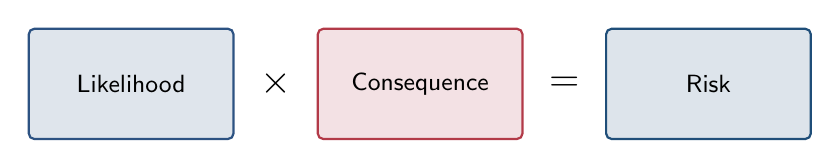
\begin{tikzpicture}[node distance=4mm]
  \node[isbox, fill=isPLC!15, draw=isPLC, minimum width=26mm, minimum height=14mm] (lik) {Likelihood};
  \node[font=\Large\bfseries, right=2mm of lik] (mul) {$\times$};
  \node[isbox, fill=isAttack!15, draw=isAttack, minimum width=26mm, minimum height=14mm, right=2mm of mul] (cons) {Consequence};
  \node[font=\Large\bfseries, right=2mm of cons] (eq) {$=$};
  \node[isbox, fill=isOT!15, draw=isOT, minimum width=26mm, minimum height=14mm, right=2mm of eq] (risk) {Risk};
\end{tikzpicture}
\vspace{3mm}
\begin{notebox}{Consequence dimensions}
\textbf{Safety}, environment, production loss, reputation, regulatory.\\
Likelihood depends on adversary capability \emph{and} exploit difficulty.
\end{notebox}
\note{
  Open by underlining that OT risk is \emph{non-linear}: once consequence reaches the safety or environmental tier, no amount of low likelihood makes the residual risk acceptable. The product form $L \times C$ is a teaching aid, not a physical law --- regulators (Seveso~III, IEC~61511) require you to drive safety risk down regardless of likelihood. Contrast with classic IT risk, where confidentiality breaches scale roughly linearly with exposure. Ask the room: what happens to this equation when $C$ contains a fatality? (Answer: the multiplication collapses --- the consequence axis dominates.) Transition: ``so how do practitioners actually plot this?''
}
\end{frame}

\begin{frame}{Risk Matrix (5$\times$5)}
\vspace{4mm}
\centering
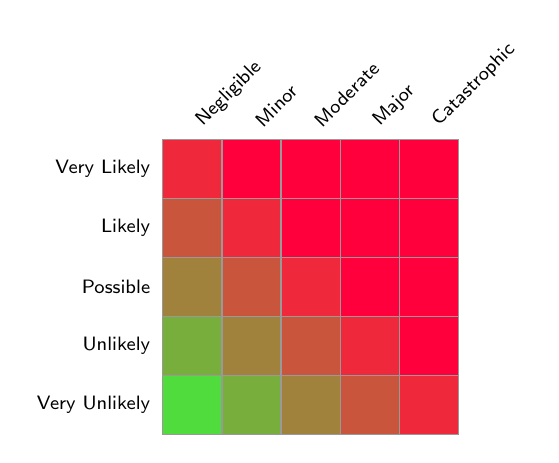
\begin{tikzpicture}[scale=0.75]
  \foreach \r/\rlbl in {0/{Very Unlikely}, 1/{Unlikely}, 2/{Possible}, 3/{Likely}, 4/{Very Likely}}{
    \node[font=\scriptsize, anchor=east] at (-0.05, \r+0.5) {\rlbl};
  }
  \foreach \c/\clbl in {0/{Negligible}, 1/{Minor}, 2/{Moderate}, 3/{Major}, 4/{Catastrophic}}{
    \node[font=\scriptsize, anchor=west, rotate=45] at (\c+0.5, 5.15) {\clbl};
  }
  \foreach \r in {0,1,2,3,4}{
    \foreach \c in {0,1,2,3,4}{
      \pgfmathtruncatemacro{\score}{\r+\c}
      \pgfmathtruncatemacro{\rr}{min(255, 80+\score*40)}
      \pgfmathtruncatemacro{\gg}{max(0, 220-\score*45)}
      \definecolor{rmcol}{RGB}{\rr,\gg,60}
      \draw[fill=rmcol, draw=black!40] (\c,\r) rectangle ++(1,1);
    }
  }
\end{tikzpicture}
\par\vspace{2mm}
\footnotesize Useful for quick communication; risk of false precision and gaming.
\note{
  Make the misconception explicit: ``a risk matrix is objective'' --- no, the \emph{colour bands are policy}. Two companies can use the same 5$\times$5 grid and disagree on which cells are red because they have different appetites. NIST~SP~800-30~R1 and ISO~31000:2018 both call out this calibration step. Common failure modes: cell-creep (analysts move scores left to escape red), category-stuffing (one ``major'' bucket that swallows everything from 1~h downtime to a fatality). Ask: ``who in your organisation owns the colour scheme?'' --- usually nobody, which is the problem. Transition: ``let's look at methods that surface the underlying logic.''
}
\end{frame}

\section{Methodologies}

\begin{frame}{Bow-Tie Analysis}
\centering
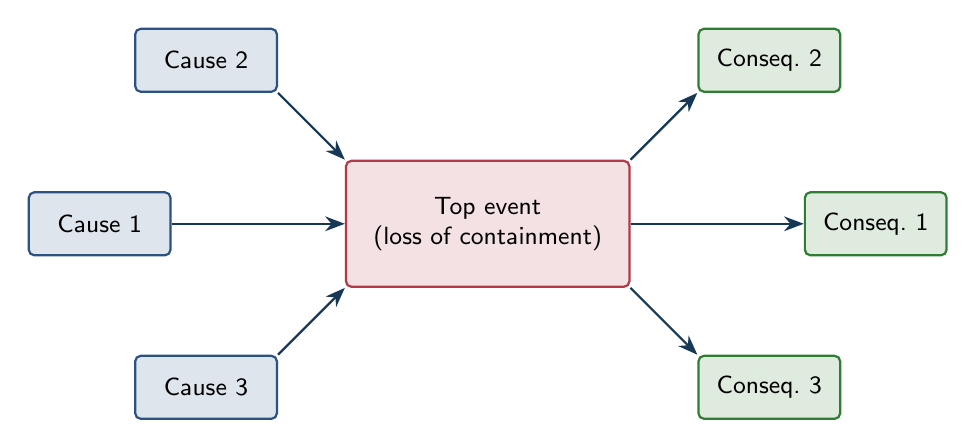
\begin{tikzpicture}[node distance=12mm]
  \node[isbox, fill=isAttack!15, draw=isAttack, minimum width=36mm, minimum height=16mm, align=center] (event) {Top event\\(loss of containment)};
  \node[isbox, fill=isPLC!15, draw=isPLC, left=22mm of event] (c1) {Cause 1};
  \node[isbox, fill=isPLC!15, draw=isPLC, above left=of event] (c2) {Cause 2};
  \node[isbox, fill=isPLC!15, draw=isPLC, below left=of event] (c3) {Cause 3};
  \node[isbox, fill=isNet!15, draw=isNet, right=22mm of event] (e1) {Conseq.\ 1};
  \node[isbox, fill=isNet!15, draw=isNet, above right=of event] (e2) {Conseq.\ 2};
  \node[isbox, fill=isNet!15, draw=isNet, below right=of event] (e3) {Conseq.\ 3};
  \draw[flow] (c1.east) -- (event.west);
  \draw[flow] (c2.south east) -- (event.north west);
  \draw[flow] (c3.north east) -- (event.south west);
  \draw[flow] (event.east) -- (e1.west);
  \draw[flow] (event.north east) -- (e2.south west);
  \draw[flow] (event.south east) -- (e3.north west);
\end{tikzpicture}
\par\vspace{2mm}
\footnotesize Barriers on the left prevent causes; barriers on the right mitigate consequences.
\note{
  The bow-tie is the diagram process-safety engineers already understand --- which makes it the right onboarding tool for security people walking into a HAZOP room. The knot in the middle is the \emph{top event} (loss of containment, runaway reaction, loss of view). Left side: threat paths and the barriers that stop them. Right side: consequence paths and the mitigations that limit damage. Stress that a \emph{cyber} cause sits on the left like any other --- ``attacker writes setpoint'' is just another initiating event. Transition: ``HAZOP gives us the verb list to walk these causes systematically.''
}
\end{frame}

\begin{frame}{Cyber-PHA / Cyber-HAZOP}
\centering
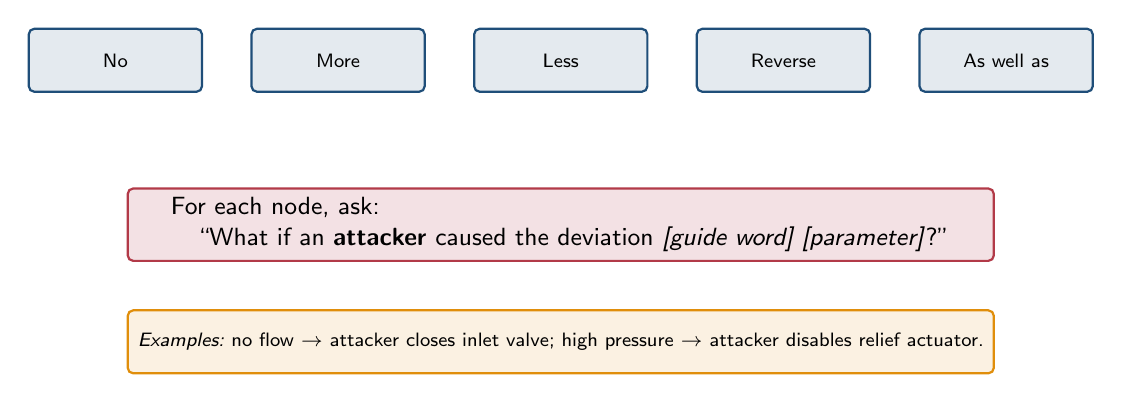
\begin{tikzpicture}[node distance=6mm]
  \node[isbox, fill=isOT!12, draw=isOT, minimum width=22mm, font=\scriptsize] (g1) {No};
  \node[isbox, fill=isOT!12, draw=isOT, minimum width=22mm, font=\scriptsize, right=of g1] (g2) {More};
  \node[isbox, fill=isOT!12, draw=isOT, minimum width=22mm, font=\scriptsize, right=of g2] (g3) {Less};
  \node[isbox, fill=isOT!12, draw=isOT, minimum width=22mm, font=\scriptsize, right=of g3] (g4) {Reverse};
  \node[isbox, fill=isOT!12, draw=isOT, minimum width=22mm, font=\scriptsize, right=of g4] (g5) {As well as};
  \node[isbox, fill=isAttack!15, draw=isAttack, minimum width=110mm, below=12mm of g3, align=left, font=\small]
    (q)
    {For each node, ask:\\
     \quad ``What if an \textbf{attacker} caused the deviation \emph{[guide word] [parameter]}?''};
  \node[isbox, fill=isAccent!12, draw=isAccent, minimum width=110mm, below=of q, align=left, font=\scriptsize]
    (ex)
    {\emph{Examples:} no flow $\to$ attacker closes inlet valve; high pressure $\to$ attacker disables relief actuator.};
\end{tikzpicture}
\source{IEC 61882:2016 (HAZOP) \textbar{} ISA TR84.00.09 (Cybersecurity for SIS).}
\note{
  Cyber-HAZOP reuses the IEC~61882 guide words but adds an adversarial mind --- not ``what if the valve sticks open?'' but ``what if the attacker \emph{holds} the valve open and spoofs the feedback?'' ISA~TR84.00.09:2017 codifies this as the bridge between functional safety (IEC~61511) and security (IEC~62443). The workshop must include a process engineer, an instrumentation engineer, and a security analyst --- otherwise you get either fantasy attacks or hand-wavy consequences. The output is a list of cyber-induced deviations that feed straight into the LOPA worksheet. Ask: ``which guide word is hardest for an attacker?'' --- usually ``reverse'', because most attackers want a one-way bad state, not an oscillation.
}
\end{frame}

\begin{frame}{Layers of Protection (LOPA)}
\centering
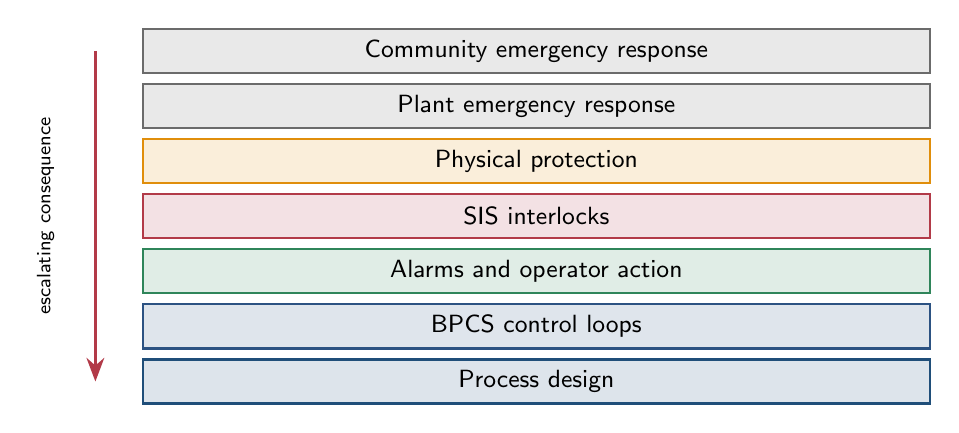
\begin{tikzpicture}[y=0.7cm]
  \foreach \r/\name/\col in {
    0/{Process design}/isOT,
    1/{BPCS control loops}/isPLC,
    2/{Alarms and operator action}/isHMI,
    3/{SIS interlocks}/isAttack,
    4/{Physical protection}/isAccent,
    5/{Plant emergency response}/isMute,
    6/{Community emergency response}/isMute}{
    \draw[fill=\col!15, draw=\col, thick] (0,\r) rectangle (10, \r+0.8);
    \node[font=\small] at (5, \r+0.4) {\name};
  }
  \draw[-{Stealth[length=3mm]}, very thick, isAttack] (-0.6,6.4) -- (-0.6, 0.4);
  \node[rotate=90, font=\scriptsize, anchor=south] at (-1.0, 3.4) {escalating consequence};
\end{tikzpicture}
\note{
  Walk top to bottom: each layer is a chance for the incident to be stopped before it escalates. The arrow on the left says ``if all seven fail, the community is exposed.'' This is the CCPS framing used in chemicals, refining, and LNG. Pre-empt the false-precision trap --- LOPA gives a number but the number is only as good as the credit you assign each layer. Ask the room: which of these layers does cyber neutralise simultaneously? (Answer: anything that runs on the same DCS --- BPCS, alarms, and an unhardened SIS can all collapse to a single common-cause cyber failure.) Transition: ``next slide quantifies that intuition.''
}
\end{frame}

\begin{frame}{Consequence-Driven Cyber-Informed Engineering (CCE)}
\vspace{-4mm}
\centering
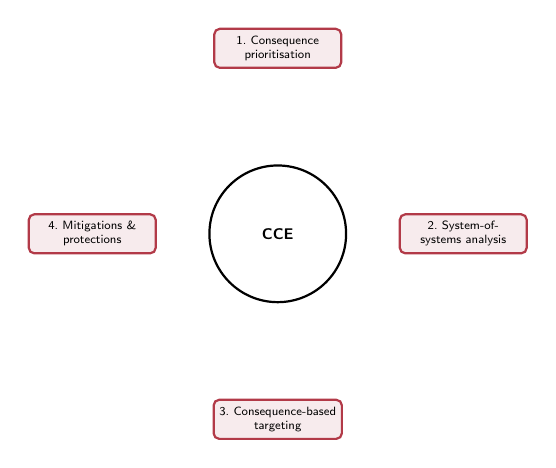
\begin{tikzpicture}[scale=0.62, transform shape]
  \def\R{1.4}
  \draw[thick] (0,0) circle (\R);
  \node[font=\bfseries\small] at (0,0) {CCE};
  \node[isbox, fill=isAttack!10, draw=isAttack, font=\scriptsize, align=center, minimum width=26mm]
    at (90:\R+2.4) {1. Consequence\\prioritisation};
  \node[isbox, fill=isAttack!10, draw=isAttack, font=\scriptsize, align=center, minimum width=26mm]
    at (0:\R+2.4) {2. System-of-\\systems analysis};
  \node[isbox, fill=isAttack!10, draw=isAttack, font=\scriptsize, align=center, minimum width=26mm]
    at (270:\R+2.4) {3. Consequence-based\\targeting};
  \node[isbox, fill=isAttack!10, draw=isAttack, font=\scriptsize, align=center, minimum width=26mm]
    at (180:\R+2.4) {4. Mitigations \&\\protections};
\end{tikzpicture}
\vspace{-1mm}
\begin{notebox}{INL methodology}
``What would I do if I were the adversary?'' \ Engineer out the worst consequences.
\end{notebox}
\source{A.\ Bochman, S.\ Freeman, \emph{Countering Cyber Sabotage}, INL/CRC Press, 2021.}
\note{
  This is the slide I want them to remember. Frame it as a single question: \emph{``if you were the adversary, what would you do?''} --- and then engineer that move \emph{out}, not just monitor for it. Idaho National Laboratory developed CCE after concluding that perimeter security alone cannot stop a determined nation-state. Phase~1 prioritises the handful of consequences the business cannot survive (typically two or three, not twenty). Phase~3 is the uncomfortable one: you red-team your own crown jewels and find the kill chain that actually works. Tell them: ``most companies do steps~1 and~4 and skip 2 and 3 --- which is why they keep being surprised.''
}
\end{frame}

\begin{frame}{Risk Response Options}
\centering
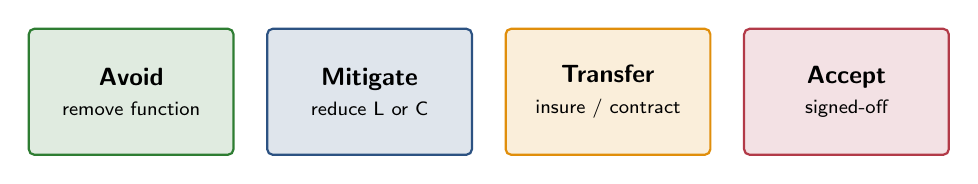
\begin{tikzpicture}[node distance=4mm]
  \node[isbox, fill=isNet!15, draw=isNet, minimum width=26mm, minimum height=16mm, align=center] (av) {\textbf{Avoid}\\\scriptsize remove function};
  \node[isbox, fill=isPLC!15, draw=isPLC, minimum width=26mm, minimum height=16mm, align=center, right=of av] (mi) {\textbf{Mitigate}\\\scriptsize reduce L or C};
  \node[isbox, fill=isAccent!15, draw=isAccent, minimum width=26mm, minimum height=16mm, align=center, right=of mi] (tr) {\textbf{Transfer}\\\scriptsize insure / contract};
  \node[isbox, fill=isAttack!15, draw=isAttack, minimum width=26mm, minimum height=16mm, align=center, right=of tr] (ac) {\textbf{Accept}\\\scriptsize signed-off};
\end{tikzpicture}
\par\vspace{2mm}
\begin{notebox}{Acceptance is legitimate}
But it must be reviewed periodically -- threats evolve.
\end{notebox}
\note{
  ISO~31000:2018 lists these four canonical responses. Stress that \emph{avoidance} is underused in OT --- if a function is risky and not load-bearing, remove it (do you really need that remote-engineering VPN to the Siemens S7?). Mitigation is the daily bread of security teams. Transfer is where insurance lives --- and it does \emph{not} reduce the underlying probability of harm. Acceptance must be a signed, time-bounded decision by someone with budget authority, not a default. Ask: ``which of these does a CISO actually have authority over?'' --- usually only mitigation and acceptance; avoidance needs the COO.
}
\end{frame}

\begin{frame}{FAIR -- Quantitative Cyber Risk}
\centering
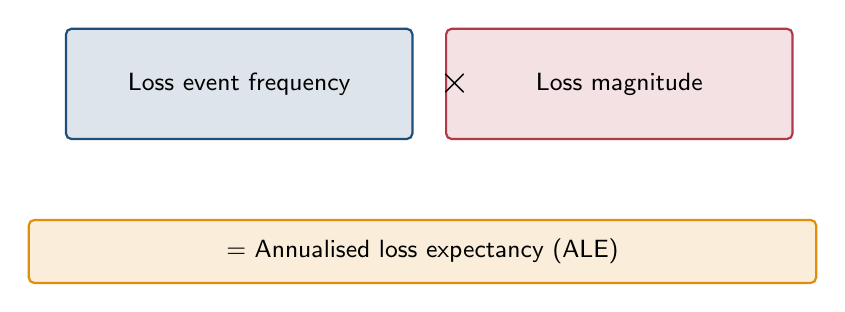
\begin{tikzpicture}[node distance=4mm]
  \node[isbox, fill=isOT!15, draw=isOT, minimum width=44mm, minimum height=14mm, align=center, font=\small] (lef) {Loss event frequency};
  \node[isbox, fill=isAttack!15, draw=isAttack, minimum width=44mm, minimum height=14mm, align=center, font=\small, right=of lef] (mag) {Loss magnitude};
  \node[font=\Large\bfseries, right=2mm of lef] {$\times$};
  \node[isbox, fill=isAccent!15, draw=isAccent, minimum width=100mm, font=\small, below=10mm of mag, xshift=-25mm] (out) {= Annualised loss expectancy (ALE)};
\end{tikzpicture}
\vspace{2mm}
\begin{notebox}{When FAIR earns its keep}
When the board asks ``how much does this risk actually cost us?'' -- and a heat-map is no longer enough.
\end{notebox}
\source{The Open Group, \emph{Risk Analysis (O-RA) Standard} (FAIR), C20A:2021 \textbar{} J.\ Jones \& J.\ Freund, \emph{Measuring and Managing Information Risk}, 2014.}
\note{
  FAIR (Factor Analysis of Information Risk) decomposes risk into measurable factors with confidence intervals --- not point estimates. The Open Group's O-RA standard formalises it. Where it earns its keep: capex justification, insurance renewal, board-level conversations where ``high / medium / low'' has stopped landing. Where it fails: when applied to safety-critical systems with sparse incident data --- you end up with a confident-looking number sitting on top of guesses. NIST~SP~800-30~R1 explicitly endorses semi-quantitative methods for exactly this reason. Ask: ``would you bet your job on the ALE figure?'' --- if not, treat it as a directional signal, not truth.
}
\end{frame}

\begin{frame}{LOPA -- Independent Protection Layers}
\centering
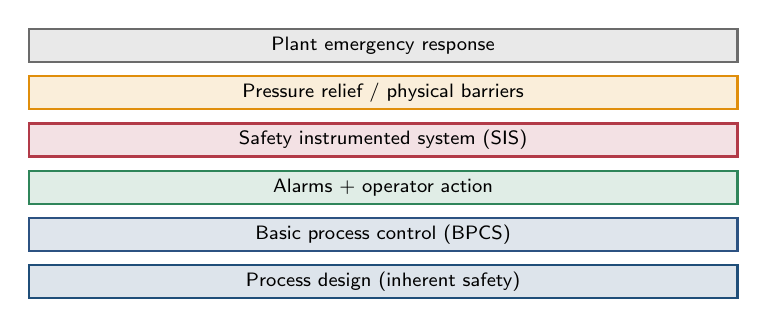
\begin{tikzpicture}[y=0.6cm]
  \foreach \r/\name/\col in {
    0/{Process design (inherent safety)}/isOT,
    1/{Basic process control (BPCS)}/isPLC,
    2/{Alarms + operator action}/isHMI,
    3/{Safety instrumented system (SIS)}/isAttack,
    4/{Pressure relief / physical barriers}/isAccent,
    5/{Plant emergency response}/isMute}{
    \draw[fill=\col!15, draw=\col, thick] (0,\r) rectangle (9, \r+0.7);
    \node[font=\scriptsize] at (4.5, \r+0.35) {\name};
  }
\end{tikzpicture}
\vspace{1mm}
\begin{notebox}{Independence is the value}
Each layer must be \emph{independent of the next} -- otherwise one common-cause failure removes them all.
\end{notebox}
\source{CCPS, \emph{Layer of Protection Analysis: Simplified Process Risk Assessment}, AIChE, 2001.}
\note{
  The point of LOPA is that probability and consequence are not the same axis. Walk through one row of the example: an attacker who can change a setpoint may, after several independent layers of protection, eventually cause a release. Each layer is a probability of failure on demand (PFD) --- typically $10^{-1}$ to $10^{-2}$ --- multiplied together. \emph{Independence} is the single most violated assumption: if your SIS shares Windows engineering workstations with the BPCS, the layers are no longer independent and the math is wrong. IEC~61511 mandates this independence for safety-rated layers. Ask: which of these layers does cyber neutralise simultaneously? (Answer: anything that runs on the same DCS.)
}
\end{frame}

\begin{frame}{Bow-Tie Example -- Loss of Containment}
\centering
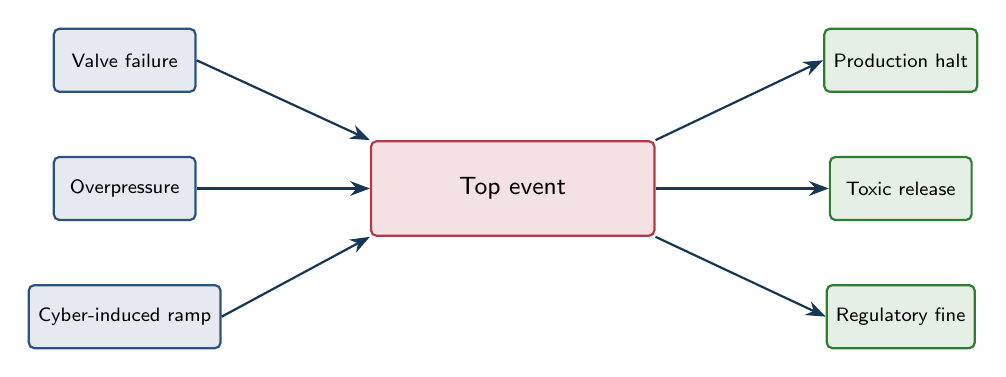
\begin{tikzpicture}[node distance=8mm]
  \node[isbox, fill=isAttack!15, draw=isAttack, minimum width=36mm, minimum height=12mm, align=center, font=\small] (e) {Top event};
  \node[isbox, fill=isPLC!12, draw=isPLC, font=\scriptsize, left=22mm of e] (c1) {Overpressure};
  \node[isbox, fill=isPLC!12, draw=isPLC, font=\scriptsize, above=of c1] (c2) {Valve failure};
  \node[isbox, fill=isPLC!12, draw=isPLC, font=\scriptsize, below=of c1] (c3) {Cyber-induced ramp};
  \node[isbox, fill=isNet!12, draw=isNet, font=\scriptsize, right=22mm of e] (k1) {Toxic release};
  \node[isbox, fill=isNet!12, draw=isNet, font=\scriptsize, above=of k1] (k2) {Production halt};
  \node[isbox, fill=isNet!12, draw=isNet, font=\scriptsize, below=of k1] (k3) {Regulatory fine};
  \draw[flow] (c1.east) -- (e.west);
  \draw[flow] (c2.east) -- (e.north west);
  \draw[flow] (c3.east) -- (e.south west);
  \draw[flow] (e.east) -- (k1.west);
  \draw[flow] (e.north east) -- (k2.west);
  \draw[flow] (e.south east) -- (k3.west);
\end{tikzpicture}
\par\vspace{1mm}
{\footnotesize Barriers on the left prevent causes; barriers on the right mitigate consequences.}
\note{
  Concrete example to make bow-tie click: pick the cyber-induced ramp on the bottom-left. Walk left-to-right: attacker writes a slow setpoint ramp, BPCS executes obediently, alarms suppressed because the rate is below threshold, SIS not tripped because the value stays under the trip point until too late --- top event reached. Right side: toxic release, production halt, regulatory fine. Now ask the room to nominate \emph{barriers}: rate-of-change alarm independent of BPCS, change-management on setpoints, signed downloads to the SIS. This is exactly how a Cyber-PHA workshop runs. Transition: ``every barrier is either a control we have or a control we owe.''
}
\end{frame}

\begin{frame}{Qualitative vs.\ Quantitative}
\centering
\renewcommand{\arraystretch}{1.3}
\footnotesize
\begin{tabular}{|p{3cm}|p{4.2cm}|p{4.6cm}|}
\hline
\rowcolor{slidePanel}
 & \textbf{Qualitative} & \textbf{Quantitative} \\
\hline
Speed       & Hours                       & Days to weeks \\
Data needed & Workshop + expert judgement & Frequency \& impact data \\
Output      & Heat map / risk matrix      & Loss curve in money \\
Use cases   & Initial triage              & Board / insurance / capex \\
Pitfalls    & False precision             & Garbage in $\Rightarrow$ garbage out \\
\hline
\end{tabular}
\note{
  These are not rivals --- they answer different questions for different audiences. Qualitative is right for the first pass and for the workshop where you cannot yet defend numbers. Quantitative (FAIR, Monte~Carlo, LOPA) is right when a decision turns on \emph{how much}, not \emph{how bad}. The trap on both sides is the same: pretending the output is more precise than the input. NIST~SP~800-30~R1 explicitly recommends semi-quantitative as a pragmatic middle ground. Ask: ``which would your CFO believe?'' --- usually the one with the dollar sign, even when the qualitative score is better calibrated. Transition: ``so where does all of this land --- in a register.''
}
\end{frame}

\begin{frame}{Cyber Insurance -- What It Buys}
\begin{itemize}
  \item First-party: forensics, IR retainer, business interruption.
  \item Third-party: liability, regulator response.
  \item Typical exclusions: nation-state acts of war, unpatched known CVEs, missing MFA.
  \item Insurers now drive a minimum control baseline (MFA, EDR, backups).
\end{itemize}
\begin{warnbox}{Backstop, not a control}
Insurance is a backstop. Premiums rise sharply if your baseline is weak, and ``act of war'' exclusions are tested in court each year.
\end{warnbox}
\source{Munich Re \emph{Cyber Insurance Risk Snapshot}, 2024 \textbar{} Merck v.\ Ace American (NotPetya war-exclusion ruling), New Jersey Appellate, 2022.}
\note{
  Hit the misconception head-on: ``buy insurance, problem solved'' --- no, \emph{exclusions are everything}. The Merck v.\ Ace American case (NotPetya, settled after the 2022 New Jersey ruling) is the canonical example: insurer invoked the ``hostile or warlike action'' exclusion against a state-attributed wiper. Merck eventually won on appeal, but only because the policy language was old; modern policies have rewritten war exclusions specifically to cover state-attributed cyber. Also stress: insurers now \emph{require} a control baseline (MFA, EDR, immutable backups) --- they are effectively the new compliance authority. Ask: ``does your risk register cite policy exclusions?'' --- if not, transfer is fictional.
}
\end{frame}

\begin{frame}{Risk Register Example}
\footnotesize
\setlength{\itemsep}{2pt}
\begin{itemize}
  \item \textbf{Ransomware on Historian} -- Likely / Major / \textcolor{calImportant}{\bfseries H}: immutable backups, EDR.
  \item \textbf{SIS reprogrammed by attacker} -- Unlikely / Catastrophic / \textcolor{calImportant}{\bfseries H}: key-switch + signed downloads.
  \item \textbf{Vendor account abuse} -- Possible / Major / \textcolor{calImportant}{\bfseries H}: MFA, brokered remote access, session recording.
  \item \textbf{USB-borne malware} -- Likely / Moderate / \textcolor{calWarning}{\bfseries M}: USB allow-listing, kiosk scanner.
  \item \textbf{PLC firmware CVE} -- Possible / Major / \textcolor{calWarning}{\bfseries M}: vendor patch in maintenance window; virtual patch on IPS meanwhile.
\end{itemize}
\note{
  A risk register is a living document, not a tickbox --- every row carries an owner, a control set, a residual rating, and a review date. Read one entry aloud: \emph{SIS reprogrammed by attacker} --- unlikely, but catastrophic, hence still high; mitigations are key-switch and signed downloads, both per IEC~62443-3-3. Stress that this register is the artefact regulators (NIS2, NIST~800-82~R3) actually ask to see during an inspection. Without it you cannot demonstrate that risks were considered and consciously treated. Ask the class: ``what would you add to this list for a water utility?'' --- expect chlorine dosing, SCADA poll-rate, and remote-pumping-station physical security.
}
\end{frame}

\begin{frame}{Summary -- Section \sectionNumber}
\begin{takeawaybox}{What to remember from this section}
\begin{itemize}\setlength{\itemsep}{2pt}
  \item Industrial risk has dimensions IT does not: safety, environment, regulatory.
  \item Cyber-HAZOP integrates security into the language of process safety teams.
  \item LOPA reminds us that several independent layers must fail for a disaster.
  \item CCE asks: how would the adversary win? -- and re-engineers to remove the winning move.
\end{itemize}
\end{takeawaybox}
\note{
  Close the loop: this section is the bridge between the technical sections that came before and the governance sections that follow. The CCE question --- ``if you were the adversary, what would you do?'' --- is the one I want you to leave with. Reinforce that no single methodology is sufficient: heat maps for speed, LOPA for independence math, FAIR for money, Cyber-PHA for safety language, CCE for the worst-case re-engineering. Each maps to a standard: ISO~31000, IEC~61511, O-RA/FAIR, ISA~TR84.00.09, INL CCE. Transition to the next section: ``now that we know what to defend and how badly, the next section asks \emph{who decides} --- governance and standards.''
}
\end{frame}

\referencesframe{
  \item The Open Group. \emph{Risk Analysis (O-RA) Standard}, C20A, 2021 (FAIR).
  \item Jones, J., Freund, J. \emph{Measuring and Managing Information Risk: A FAIR Approach}, Butterworth-Heinemann, 2014.
  \item Center for Chemical Process Safety (CCPS). \emph{Layer of Protection Analysis: Simplified Process Risk Assessment}, AIChE, 2001.
  \item IEC 61882:2016. \emph{Hazard and operability studies (HAZOP studies) -- Application guide}.
  \item ISA-TR84.00.09:2017. \emph{Cybersecurity related to the Functional Safety Lifecycle}.
  \item Bochman, A., Freeman, S. \emph{Countering Cyber Sabotage: Introducing Consequence-Driven, Cyber-Informed Engineering (CCE)}, INL/CRC Press, 2021.
  \item IEC 62443-3-2:2020. \emph{Security risk assessment for system design}.
  \item NIST SP 800-30 Rev.\,1. \emph{Guide for Conducting Risk Assessments}, 2012.
  \item ISO 31000:2018. \emph{Risk management -- Guidelines}.
}

\closingframe

\end{document}
